\documentclass{beamer}
\usetheme{Boadilla}
\usepackage{listings}
\usepackage{color}
\usepackage{alltt}
\usepackage{wrapfig}
\usepackage{array}
\author{Rob Stewart}
\institute{Heriot Watt University}
\title{Towards a Semantic Web Toolkit in Haskell}
\date{\emph{Updated: 29th September 2012}}
\subtitle{Querying RDF graphs \& SPARQL construction}

\newcommand{\hilightyellow}[1]{\colorbox{yellow}{#1}}
\newcommand{\hilightgreen}[1]{\colorbox{green}{#1}}
\newcommand{\hilightorange}[1]{\colorbox{orange}{#1}}
\newcommand{\hilightpink}[1]{\colorbox{pink}{#1}}

\lstdefinestyle{MyJavaStyle} {
   language=Java,
   basicstyle=\scriptsize,
   showstringspaces=false,
   breaklines=true
}


\lstloadlanguages{Haskell}
\lstnewenvironment{haskellcode}
    {\lstset{}%
      \csname lst@SetFirstLabel\endcsname}
    {\csname lst@SaveFirstLabel\endcsname}
    \lstset{
      basicstyle=\scriptsize\ttfamily,
      flexiblecolumns=false,
      basewidth={0.5em,0.45em},
      literate={+}{{$+$}}1 {/}{{$/$}}1 {*}{{$*$}}1 {=}{{$=$}}1
               {>}{{$>$}}1 {<}{{$<$}}1 {\\}{{$\lambda$}}1
               {\\\\}{{\char`\\\char`\\}}1
               {->}{{$\rightarrow$}}2 {>=}{{$\geq$}}2 {<-}{{$\leftarrow$}}2
               {<=}{{$\leq$}}2 {=>}{{$\Rightarrow$}}2 
               {\ .}{{$\circ$}}2 {\ .\ }{{$\circ$}}2
               {>>}{{>>}}2 {>>=}{{>>=}}2
               {|}{{$\mid$}}1               
    }


\begin{document}


\section{Introduction}

\maketitle

\begin{frame}[fragile]
\frametitle{Preamble}

\begin{itemize}
\item Who I am\ldots
  
  \begin{itemize}
  \item Work @ Heriot Watt University
    
    \begin{itemize}
    \item \textbf{PhD} Fault tolerant, distributed-memory Haskell computing
    \item \textbf{Researcher} SerenA project \emph{(more on that later)}.
    \end{itemize}
    
  \item I'm on Twitter: \texttt{@robstewartUK}
  \item I'm also on Google+: \texttt{http://goo.gl/eL8zg}
    
  \end{itemize}
  
\bigskip
\item What I'll talk about
  
  \begin{itemize}
  \item The \emph{semantic web}
  \item Linked Open Data
  \item Available Haskell libraries to poke at both
  \end{itemize}

\bigskip
\item LaTeX, Haskell \& Java source code on GitHub:

\small
\texttt{https://github.com/robstewart57/edlambda-semanticweb-haskell}
  
\end{itemize}

\end{frame}


\begin{frame}

\huge
\begin{center}
The Semantic Web
\end{center}

\end{frame}

\begin{frame}
\frametitle{The Semantic Web}
\framesubtitle{What is it?}

\begin{center}

\includegraphics[width=15mm]{images/swlogo.pdf}
\end{center}

\begin{itemize}
\item A collaborative movement led by W3C
\item Promotes common data formats
\item Moving from \emph{unstructured documents} into a \textbf{web of
  data}.
\item \emph{``Web 3.0''} is sometimes used as a synonym for the
  semantic web.
\end{itemize}

\begin{quotation}
The Semantic Web provides a common framework that allows data to be
shared and reused across application, enterprise, and community
boundaries \footnote{"W3C Semantic Web Activity". World Wide Web
  Consortium (W3C). November 7, 2011}.
\end{quotation}

\end{frame}

\begin{frame}
\frametitle{Future of the Web}
\framesubtitle{Web connectivity}

\begin{center}
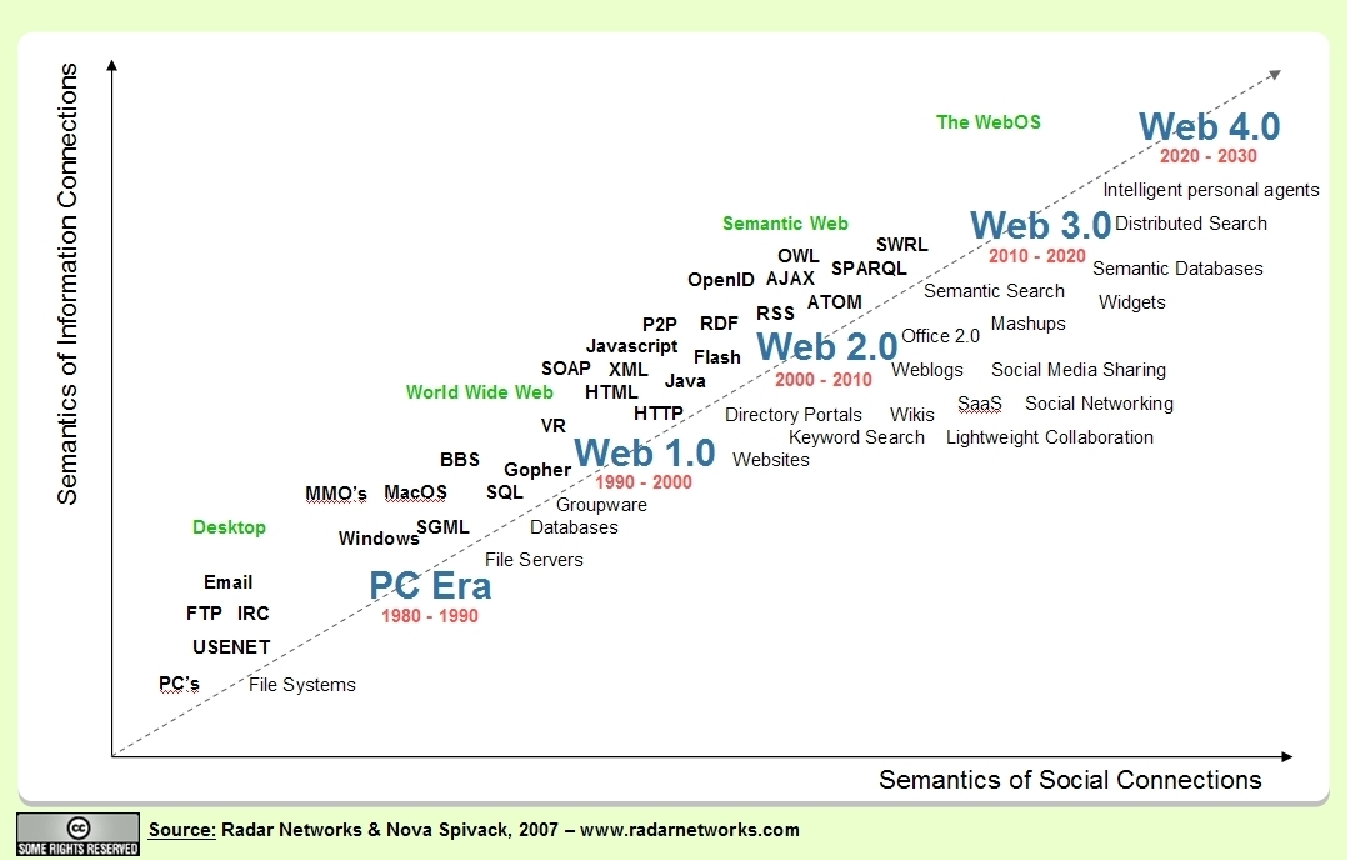
\includegraphics[width=120mm]{images/web-future.pdf}
\end{center}


\end{frame}


\begin{frame}
\frametitle{The Semantic Web}
\framesubtitle{Semantic Web Stack}

\begin{center}
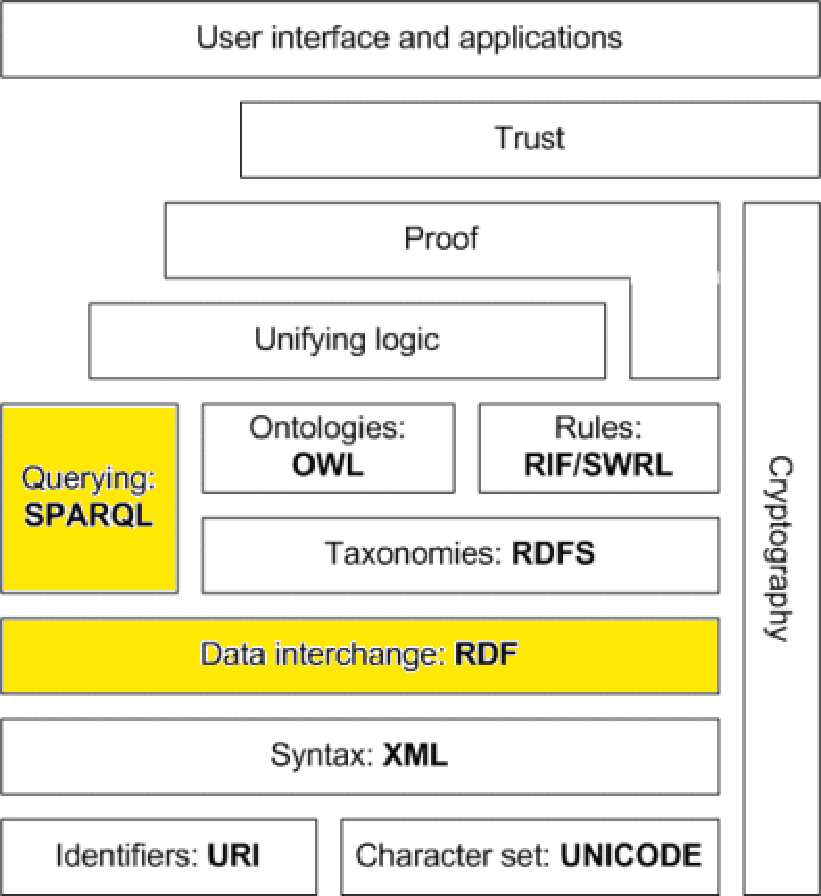
\includegraphics[width=60mm]{images/sw-stack-colour.pdf}
\end{center}

\end{frame}


\begin{frame}[fragile]
\frametitle{The Semantic Web}
\framesubtitle{Principles}

\begin{itemize}
\item \textbf{URI} is simply a Web identifier

  \begin{itemize}
  \item A disambiguation mechanism for distributed data
  \item Start with \emph{http://} or \emph{ftp://} \ldots
  \item Anyone can create a URI! e.g.

    \begin{itemize}
    \item \texttt{https://twitter.com/\#!/robstewartUK}
    \item \texttt{http://dblp.l3s.de/d2r/page/authors/Tim\_Berners-Lee} 
    \end{itemize}
  \end{itemize}

\pause

\item \textbf{RDF} statements consist of three parts:
  
  \begin{description}
  \item[Subject] is the \emph{resource} being described
  \item[Predicate] indicates a relationship with\ldots
  \item[Object] is either a resource or a \emph{literal}
  \end{description}
  
  \begin{itemize}
  \item RDF can be serialised in XML, N3, Turtle and
    JSON\footnote{though not yet standardised}.
  \end{itemize}
  
\end{itemize}

\end{frame}

\begin{frame}
\frametitle{The Semantic Web}
\framesubtitle{Two RDF triples}

\begin{center}
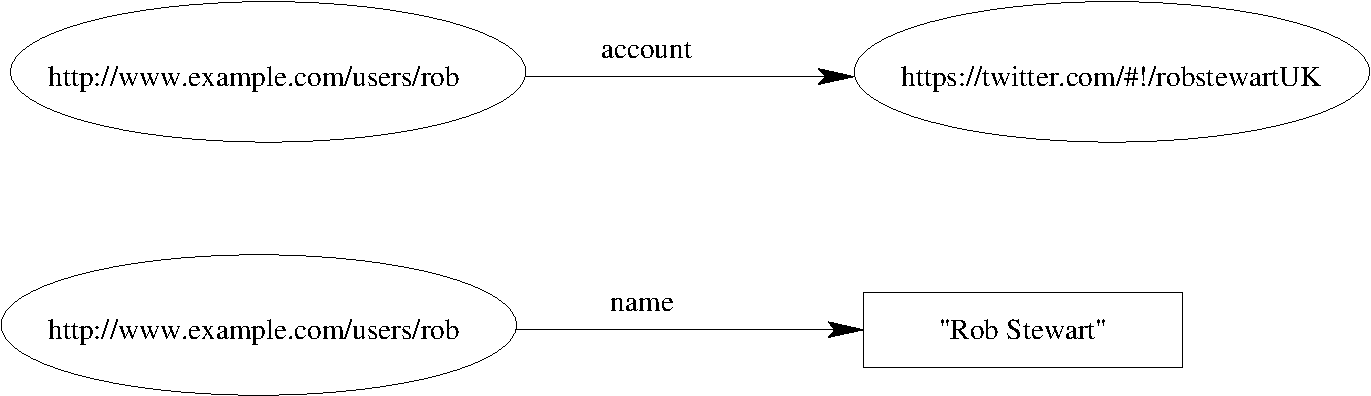
\includegraphics[width=120mm]{images/rdfexample.pdf}
\end{center}

\end{frame}




\begin{frame}[fragile]
\frametitle{The Semantic Web}
\framesubtitle{Resource Description Framework serialised in XML}

\small
\begin{alltt}
<?xml version="1.0"?>
<rdf:RDF
  xmlns:rdf="http://www.w3.org/1999/02/22-rdf-syntax-ns#"
  xmlns:foaf="http://xmlns.com/foaf/0.1/">
<rdf:RDF>
  <rdf:Description about="http://www.example.com/users/rob">
    <foaf:name>Rob Stewart</foaf:name>
    <foaf:account
       rdf:resource="https://twitter.com/#!/robstewartUK" />
  </rdf:Description>
</rdf:RDF>
\end{alltt}

\end{frame}

\begin{frame}[fragile]
\frametitle{The Semantic Web}
\framesubtitle{Resource Description Framework serialised in XML}

\small
\begin{alltt}
<?xml version="1.0"?>
<rdf:RDF
\hilightyellow{xmlns:rdf="http://www.w3.org/1999/02/22-rdf-syntax-ns#"}
\hilightyellow{xmlns:foaf="http://xmlns.com/foaf/0.1/">}
<rdf:RDF>
  \hilightgreen{<rdf:Description about="http://www.example.com/users/rob">}
    \hilightpink{<foaf:name>}\hilightorange{Rob Stewart}\hilightpink{</foaf:name>}
    \hilightpink{<foaf:account}
       \hilightorange{rdf:resource="https://twitter.com/#!/robstewartUK"}\hilightpink{/>}
  \hilightgreen{</rdf:Description>}
</rdf:RDF>
\end{alltt}

\bigskip
\textbf{Key}

\hilightyellow{Prefixes}
\hilightgreen{Subject}
\hilightpink{Predicate}
\hilightorange{Object}

\end{frame}

\begin{frame}[fragile]
\frametitle{The Semantic Web}
\framesubtitle{SPARQL}

\textbf{S}PARQL \textbf{P}rotocol \textbf{a}nd \textbf{R}DF
\textbf{Q}uery \textbf{L}anguage

\begin{itemize}
\item And RDF query language to retrieve and manipulate persisted RDF
\item On 15th January 2008, SPARQL 1.0 became W3C recommendation

  \bigskip
\item Four query forms
  
  \begin{itemize}
  \item \texttt{SELECT} Extracts raw values to a table format
  \item \texttt{CONSTRUCT} Extracts raw values into RDF
  \item \texttt{ASK} Queries for the existence of a triple
  \item \texttt{DESCRIBE} Extracts triples where specified URI is subject
  \end{itemize}
  
\end{itemize}

\end{frame}

\begin{frame}[fragile]
\frametitle{The Semantic Web}
\framesubtitle{SPARQL SELECT}


\begin{verbatim}
PREFIX foaf: <http://xmlns.com/foaf/0.1/>
SELECT ?name ?account
WHERE {
 ?person foaf:name ?name
 ?person foaf:account ?account
}
\end{verbatim}

\bigskip

\begin{center}
\begin{tabular}{| c | c | }
\hline
\textbf{name} & \textbf{account} \\
\hline
``Rob Stewart'' & $\textless$https://twitter.com/\#!/robstewartUK$\textgreater$ \\
\hline
\end{tabular}
\end{center}

\end{frame}


\begin{frame}[fragile]
\frametitle{The Semantic Web}
\framesubtitle{SPARQL DESCRIBE}


\begin{verbatim}
DESCRIBE <http://www.example.com/users/rob>
\end{verbatim}

\bigskip

\begin{center}
\small
\begin{verbatim}
<?xml version="1.0"?>
<rdf:RDF
  xmlns:rdf="http://www.w3.org/1999/02/22-rdf-syntax-ns#"
  xmlns:foaf="http://xmlns.com/foaf/0.1/">
<rdf:RDF>
  <rdf:Description about="http://www.example.com/users/rob">
    <foaf:name>Rob Stewart</foaf:name>
    <foaf:account
       rdf:resource="https://twitter.com/#!/robstewartUK" />
  </rdf:Description>
</rdf:RDF>
\end{verbatim}
\end{center}

\end{frame}


\begin{frame}[fragile]
\frametitle{The Semantic Web}
\framesubtitle{SPARQL CONSTRUCT}


\begin{verbatim}
PREFIX foaf: <http://xmlns.com/foaf/0.1/>
PREFIX example: <http://www.example.org/onto/>
CONSTRUCT { ?person example:hasName ?name }
WHERE {
  ?person foaf:name ?name
}
\end{verbatim}

\bigskip

\begin{center}
\begin{tabular}{| c | c | }
\hline
\textbf{name} & \textbf{account} \\
\hline
``Rob Stewart'' & $\textless$https://twitter.com/\#!/robstewartUK$\textgreater$ \\
\hline
\end{tabular}
\end{center}

\end{frame}


\begin{frame}[fragile]
\frametitle{The Semantic Web}
\framesubtitle{SPARQL ASK}

\small
\begin{verbatim}
PREFIX foaf: <http://xmlns.com/foaf/0.1/>
ASK { ?x foaf:name "Rob Stewart" }
\end{verbatim}

\begin{center}
\textbf{Yes.}
\end{center}

\bigskip

\small
\begin{verbatim}
PREFIX foaf: <http://xmlns.com/foaf/0.1/>
ASK {?x foaf:topic_interest
         <http://www.dbpedia.org/resource/Closed_source_software>}
\end{verbatim}

\begin{center}
\textbf{No.}
\end{center}


\end{frame}

\begin{frame}

\huge
\begin{center}
Linked Open Data
\end{center}

\end{frame}

\begin{frame}
\frametitle{Linked Open Data}
\framesubtitle{What is it?}

\begin{itemize}
\item Linked Data
  
  \begin{itemize}
  \item Semantic structured data\ldots
  \item Using semantic web principles (e.g. RDF)
  \item Referencing disambiguated URIs means data is interlinked 
  \end{itemize}
  
\pause
\item Open Data
  
  \begin{itemize}
  \item Certain data should be freely available to use and republish
  \item Without copyright, patents, or imposed control
  \item Philosophy correlates to \emph{open source code \& open access}.
  \end{itemize}
  
\pause
\item Linked Open Data!
  \begin{itemize}
  \item LOD project aims to publish open data sets as RDF. Data sources include:
    
    \begin{itemize}
    \item DBpedia
    \item Geonames
    \item MusicBrainz
    \item DBLP
    \end{itemize}
    
  \end{itemize}

\end{itemize}
\end{frame}

\begin{frame}
\frametitle{Linked Open Data}
\framesubtitle{In September 2007}

\begin{center}
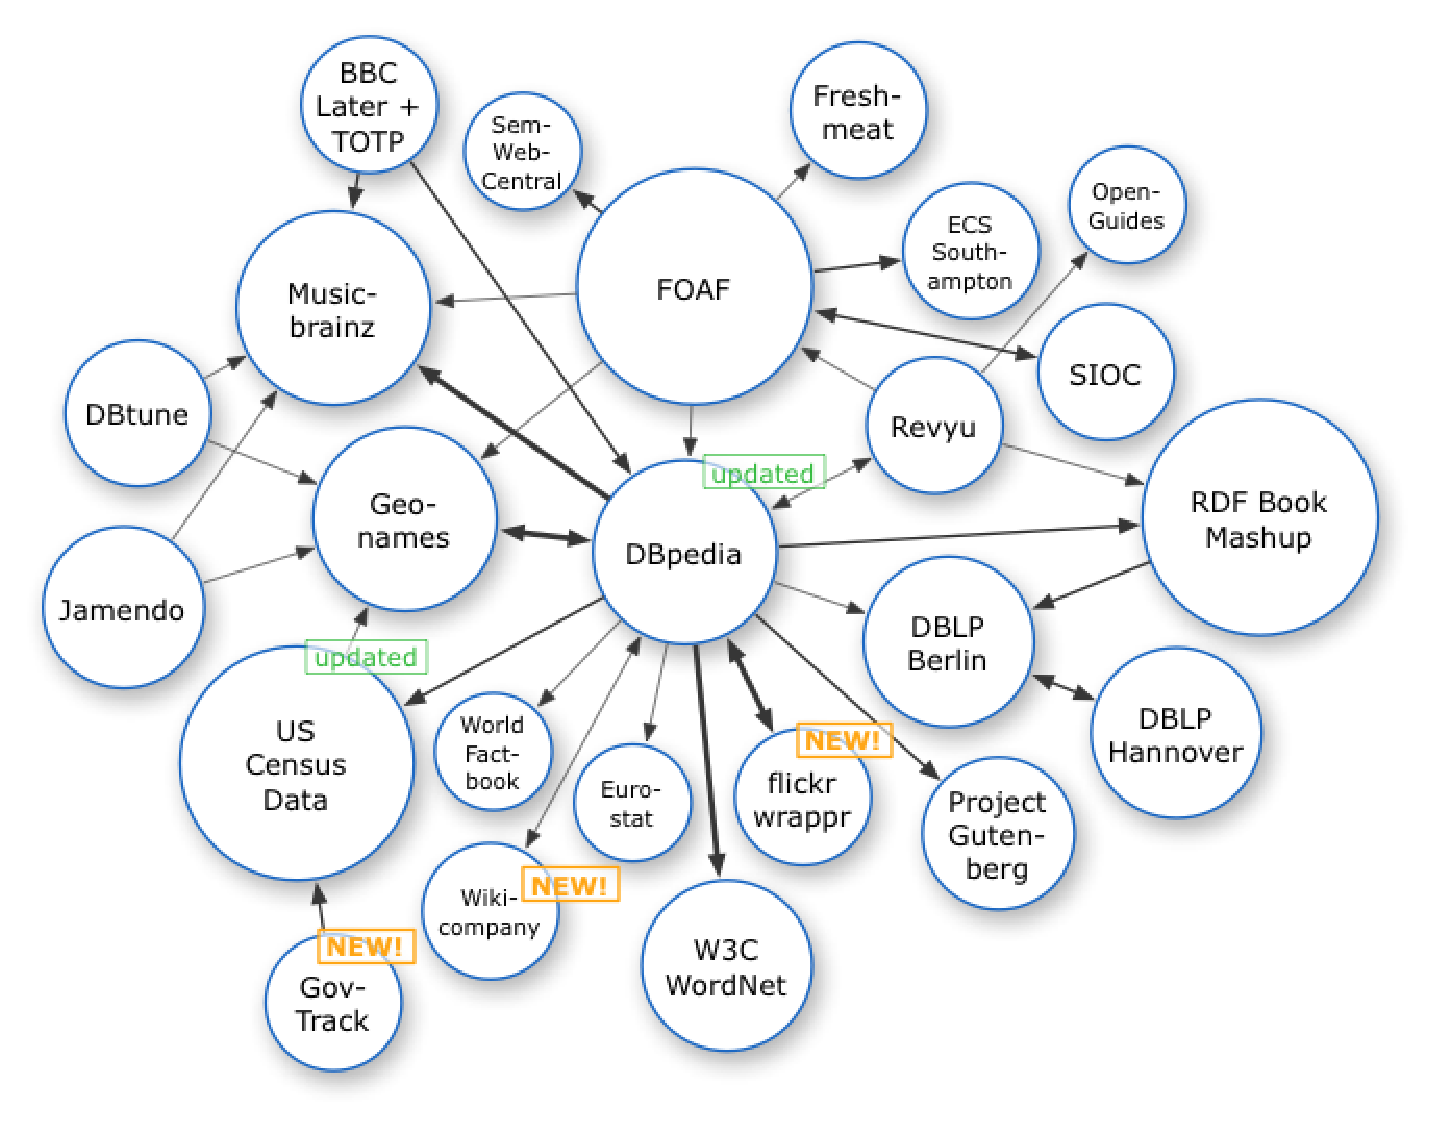
\includegraphics[width=80mm]{images/lod-2007.pdf}
\end{center}

\end{frame}

\begin{frame}
\frametitle{Linked Open Data}
\framesubtitle{In September 2011}

\begin{center}
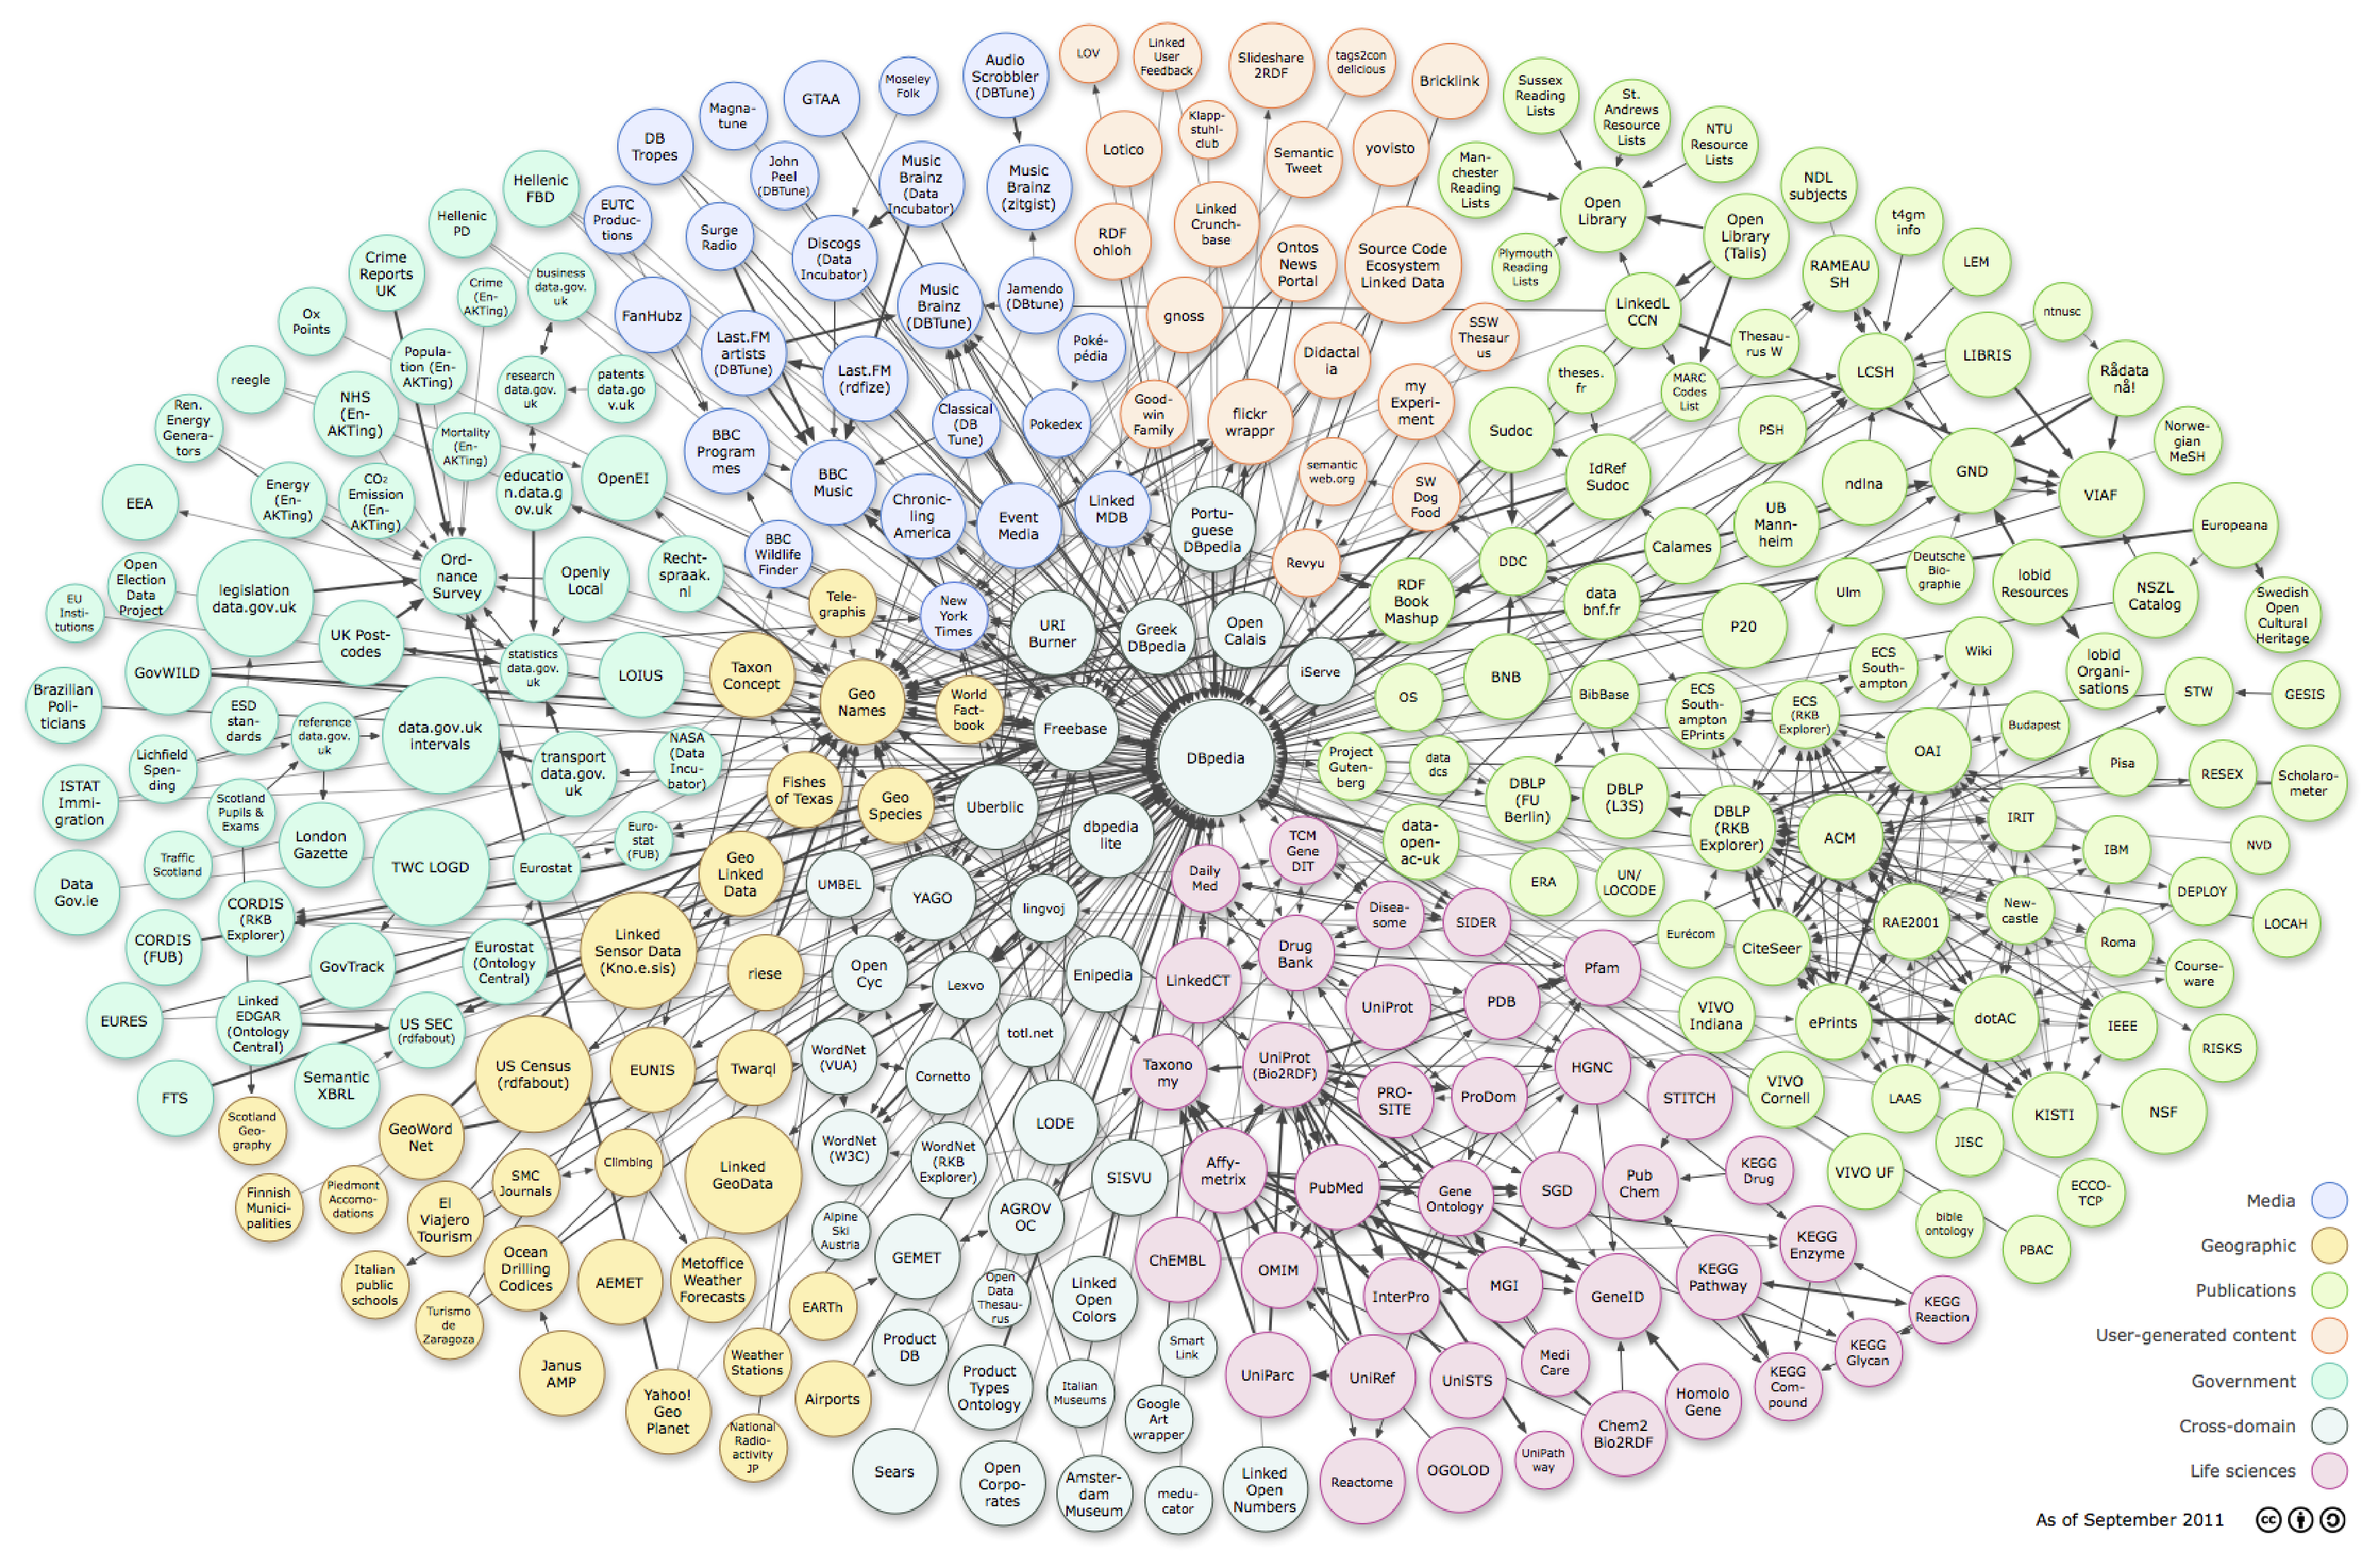
\includegraphics[width=100mm]{images/lod-2011.pdf}
\end{center}

\end{frame}


\begin{frame}
\frametitle{Linked Open Data}
\framesubtitle{What is DBpedia?}

\begin{center}
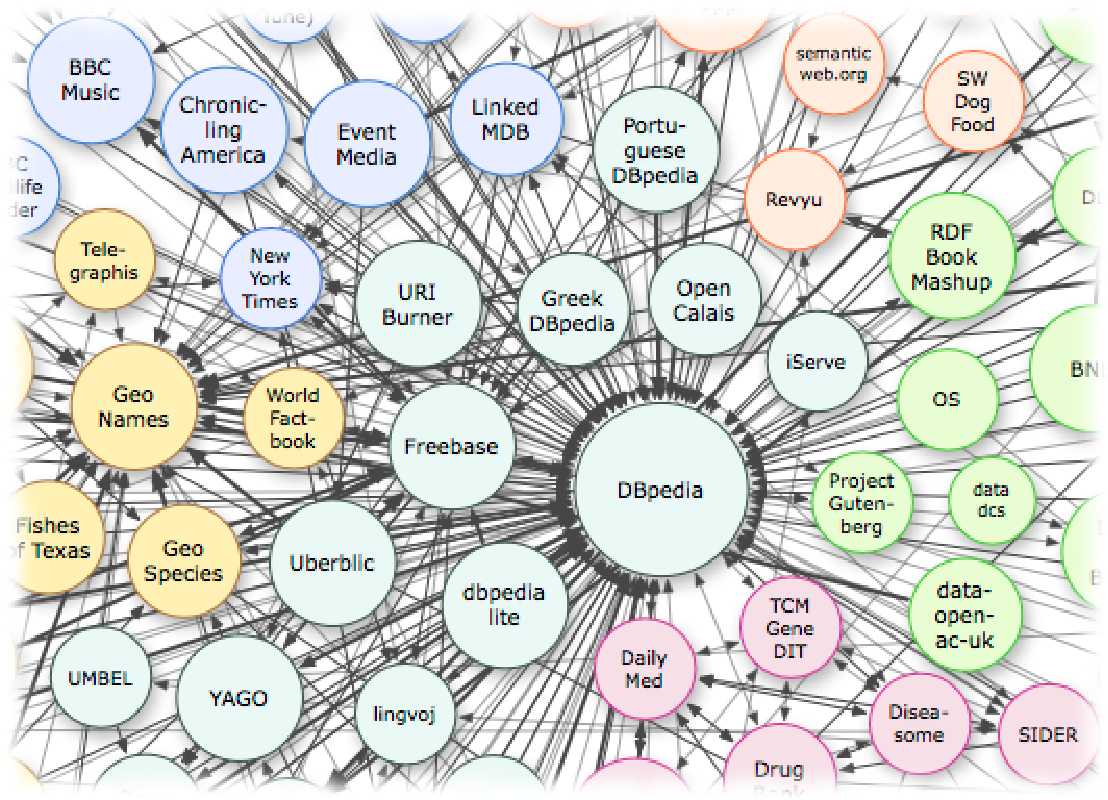
\includegraphics[width=50mm]{images/lod-2011-dbpedia.pdf}
\end{center}

\begin{itemize}
\item Extracts structured content from \emph{Wikipedia} pages.
\item Query relationships associated with Wikipedia resources\ldots
\item Including links to other semantic datasets (which is cool!).
\item Describes \emph{3.64 million} things, including\ldots

\begin{itemize}
\item \emph{416,000} persons
\item \emph{526,000} places
\item and \emph{169,000} organisations
\end{itemize}

\end{itemize}

\end{frame}

\begin{frame}
\frametitle{Linked Open Data}
\framesubtitle{Resource Example - \texttt{http://dbpedia.org/resource/Edinburgh}}

\begin{center}
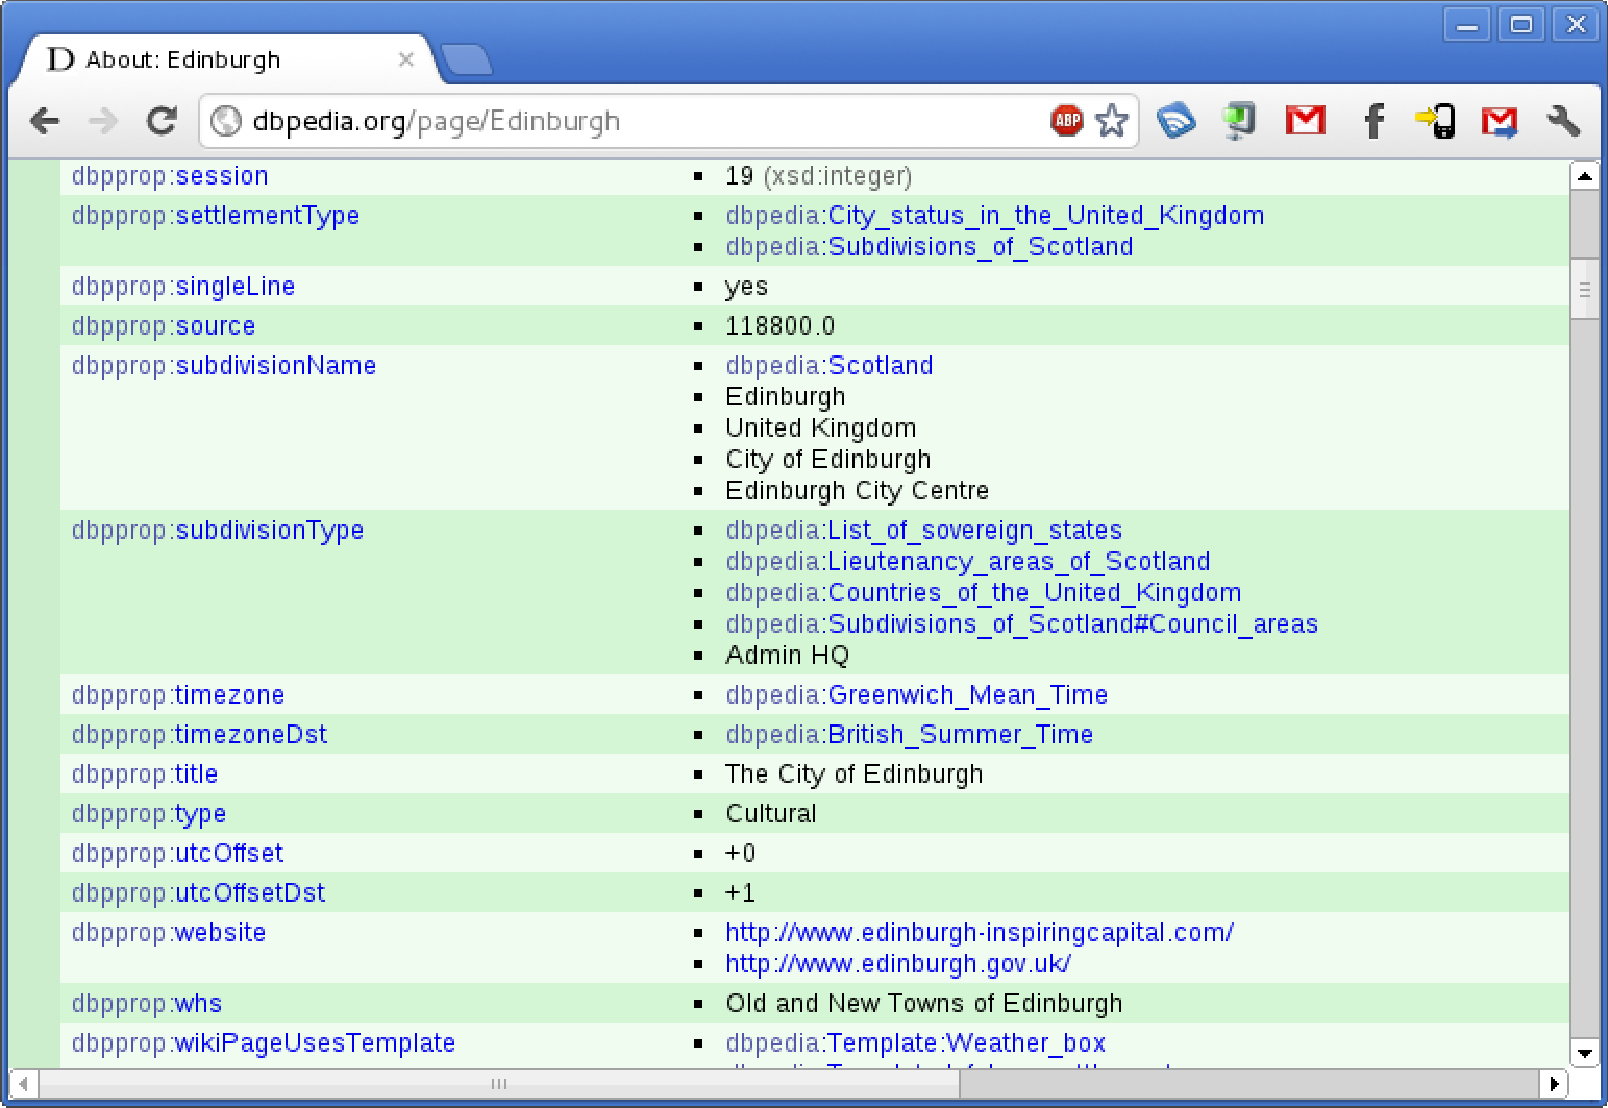
\includegraphics[width=110mm]{images/edinburgh-dbpedia.pdf}
\end{center}

\end{frame}

\begin{frame}
\frametitle{Linked Open Data}
\framesubtitle{\emph{Linked Geo Data} Project}

\begin{center}

\includegraphics[width=30mm]{images/lgdlogo.pdf}
\end{center}

\begin{itemize}
\item Effort to add spatial dimension to \emph{web of data}
\item Uses \emph{crowd sourced} information from OpenStreetMap
\item Interlinked resources with other knowledge bases on LOD network
\bigskip
\item Information of 350 million nodes and 30 million ways\ldots
\item Resulting in over 2 billion triples!
\end{itemize}

\end{frame}

\begin{frame}
\frametitle{Linked Open Data}
\framesubtitle{\emph{Linked Geo Data} Project}

\begin{center}
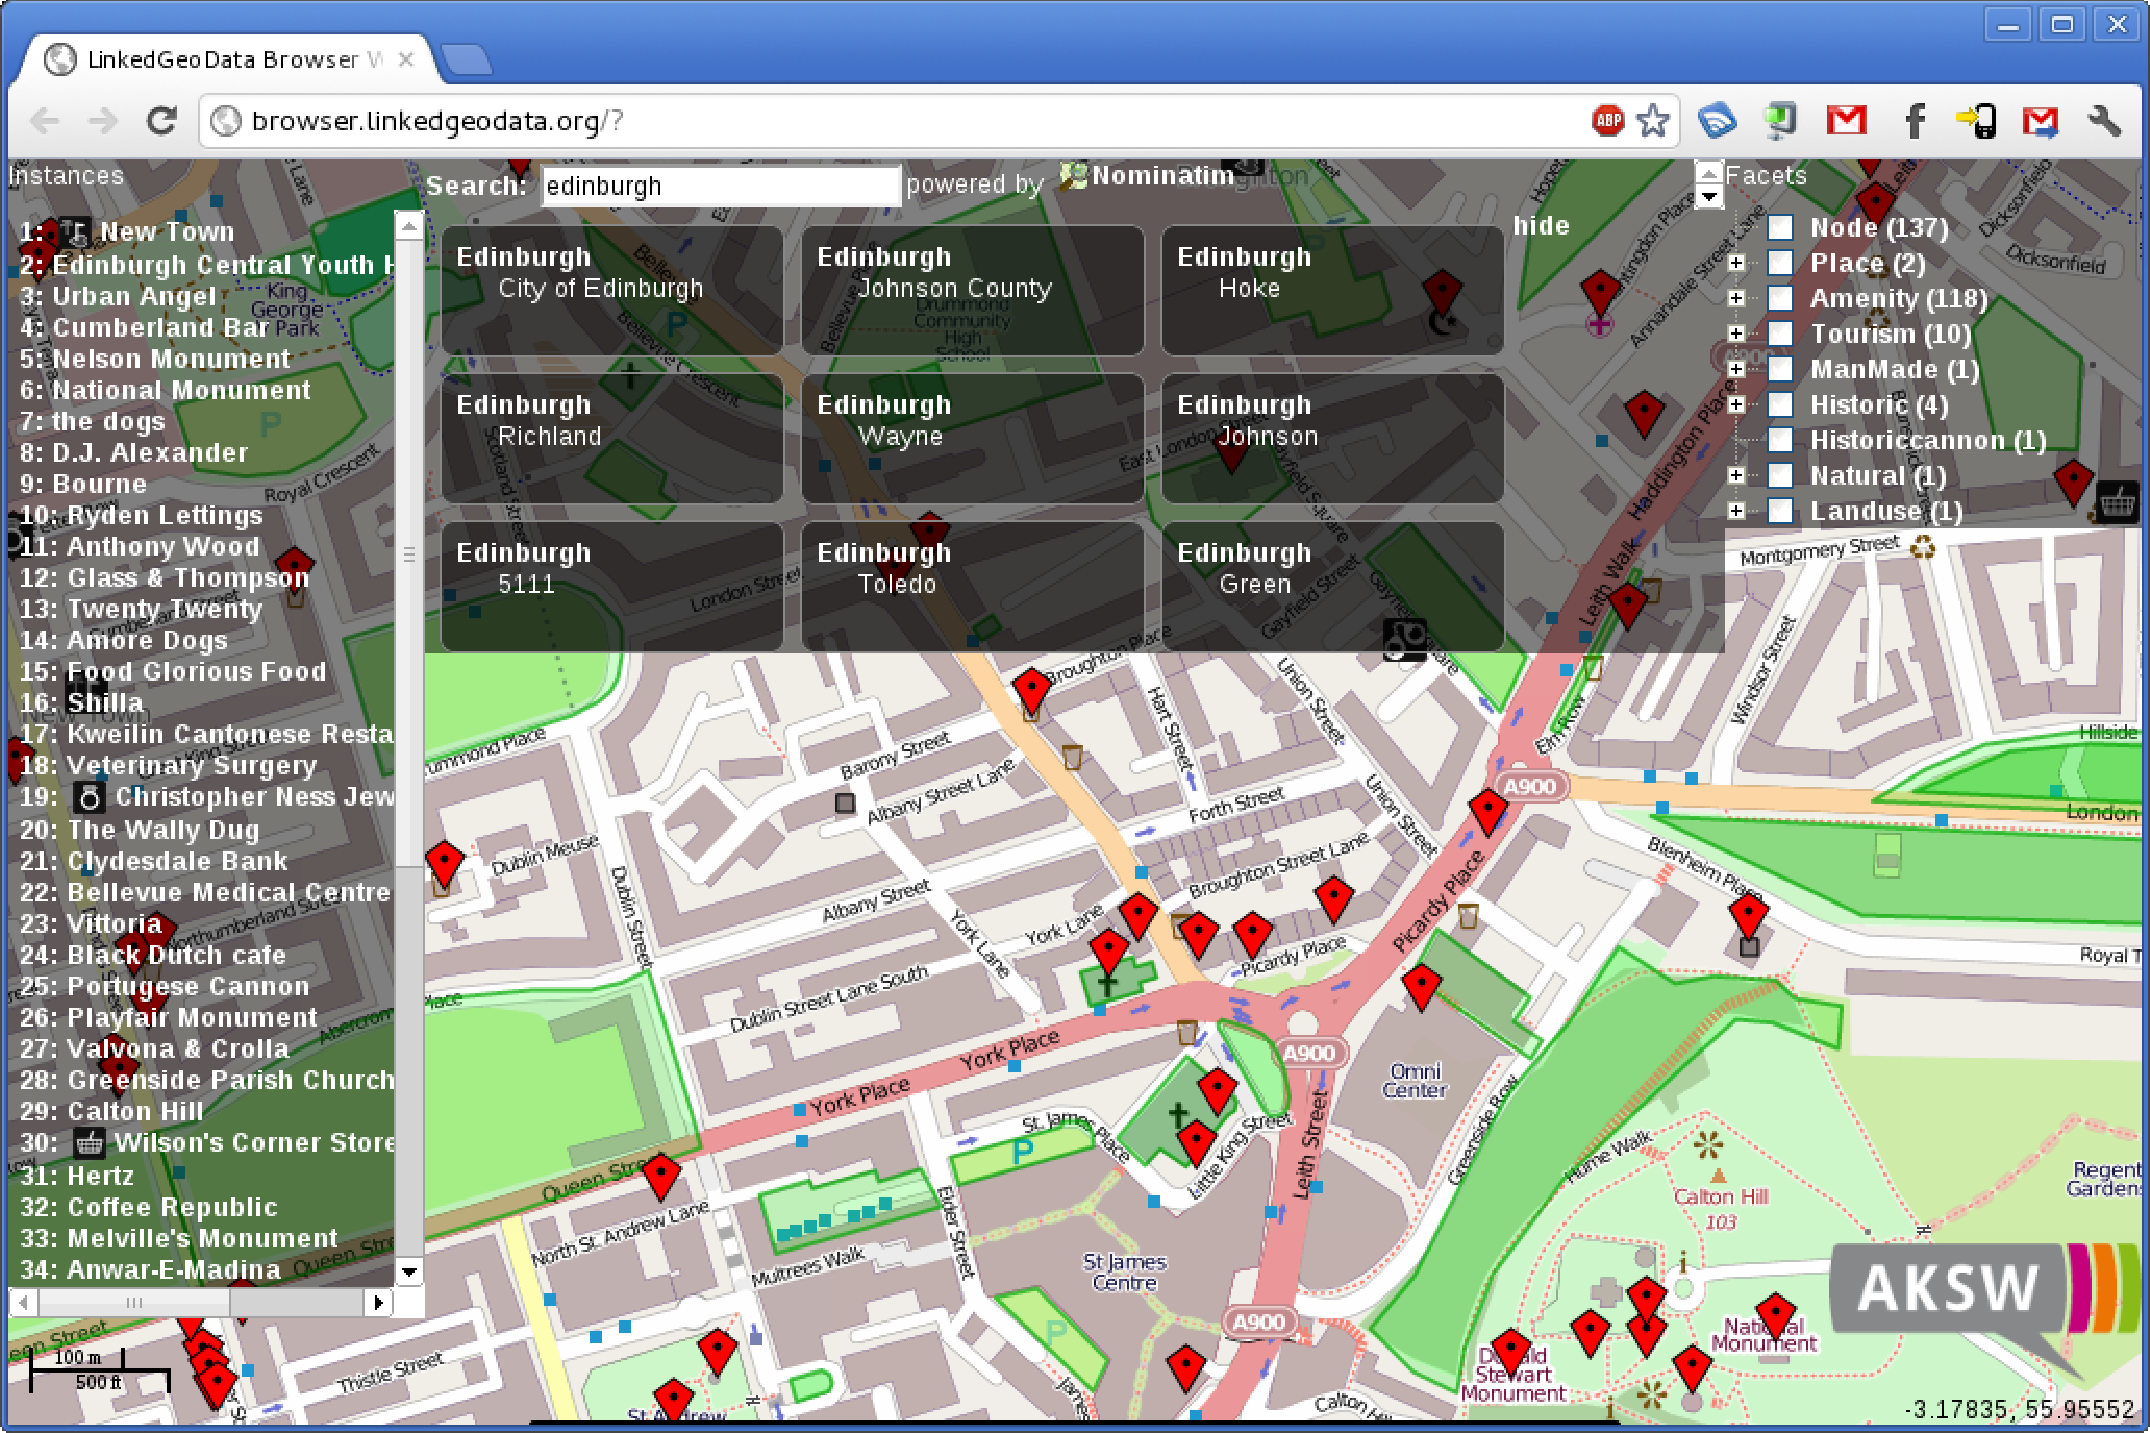
\includegraphics[width=110mm]{images/osm.pdf}
\end{center}

\end{frame}


\begin{frame}[fragile]
\frametitle{Linked Open Data - Project case study}
\framesubtitle{SerenA - \emph{Chance Encounters in the Space of Ideas}}


\begin{center}
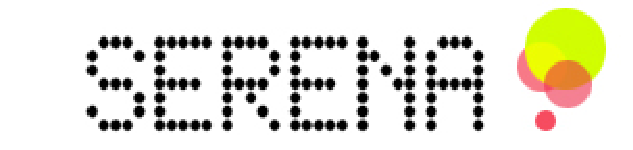
\includegraphics[width=0.4\textwidth]{images/serena-logo.pdf}
\end{center}

\begin{itemize}
\item Homepage: \texttt{http://www.serena.ac.uk}
\item Aims to bring closer people with \emph{ideas, places, relevant
  documents, people}\ldots resources!
\item Presentation of ideas and resources, plus explanation of chain
  reasoning is \emph{really} important for perceived
  \textbf{serendipity}.
\item Implementation efforts are in progress\ldots
  
  \begin{itemize}
  \item Information seeking on cloud of \emph{Linked Open Data}
  \item \emph{Agent framework} used for autonomous search and interface scheduling
  \end{itemize}
  
\end{itemize}

For more implementation info: \texttt{http://goo.gl/ZGsfJ}

\end{frame}


\begin{frame}
\frametitle{Semantic Web}
\framesubtitle{Real World Applications}

\begin{itemize}
\item \textbf{Web search}
  
  \begin{itemize}
  \item \texttt{schema.org} used by Microsoft, Google and Yahoo.

\begin{quotation}
``A shared markup vocabulary makes easier for webmasters to decide on
  a markup schema and get the maximum benefit for their efforts'' \footnote{http://schema.org/}.
\end{quotation}

  \end{itemize}
  
\item \textbf{Retail}
  
\begin{itemize}
\item \texttt{http://www.bestbuy.com}
  
  \begin{itemize}
  \item Exposes RDF describing their products
  \item 450,000 items, 60 triples per item\ldots ~27 million triples!
    

  \end{itemize}

    \begin{quotation}
``It’s easy to sell the top 20 products using keywords, but surfacing
      the long tail is where the data makes the
      difference.'' - \emph{Jay Myers}, Best Buy \footnote{Best Buy Adopts RDF and the Open Web http://goo.gl/EWar}
    \end{quotation}
    
  
  \end{itemize}
\end{itemize}

\end{frame}

\begin{frame}[fragile]
\frametitle{Semantic Web}
\framesubtitle{JISC Monitoring Unit Data as RDF}

\begin{itemize}
\item Project leader: Wilbert Kraan (\texttt{@wilm} on Twitter)
\item JISCMU\ldots

\begin{quotation}
supports JISC policy and planning by providing a quality assurance
role in monitoring the performance and use of JISC
services. \footnote{http://www.jiscmu.ac.uk/about/}
\end{quotation}

\item Example - full \emph{institute} data as RDF/XML

\begin{itemize}
\item \texttt{http://data.jiscmu.ac.uk/rest/organisations/}
\end{itemize}

\end{itemize}

\begin{center}
\line(1,0){250}
\end{center}

\begin{verbatim}
SELECT ?Institution ?p ?o
WHERE{ 
?Institution a mu:Organisation .
?Institution mu:OfficialName "University of Edinburgh" .
?Institution ?p ?o . }
\end{verbatim}

\end{frame}

\begin{frame}[fragile]
\frametitle{Semantic Web}
\framesubtitle{Linked Data: JISC Institute data}

\begin{center}
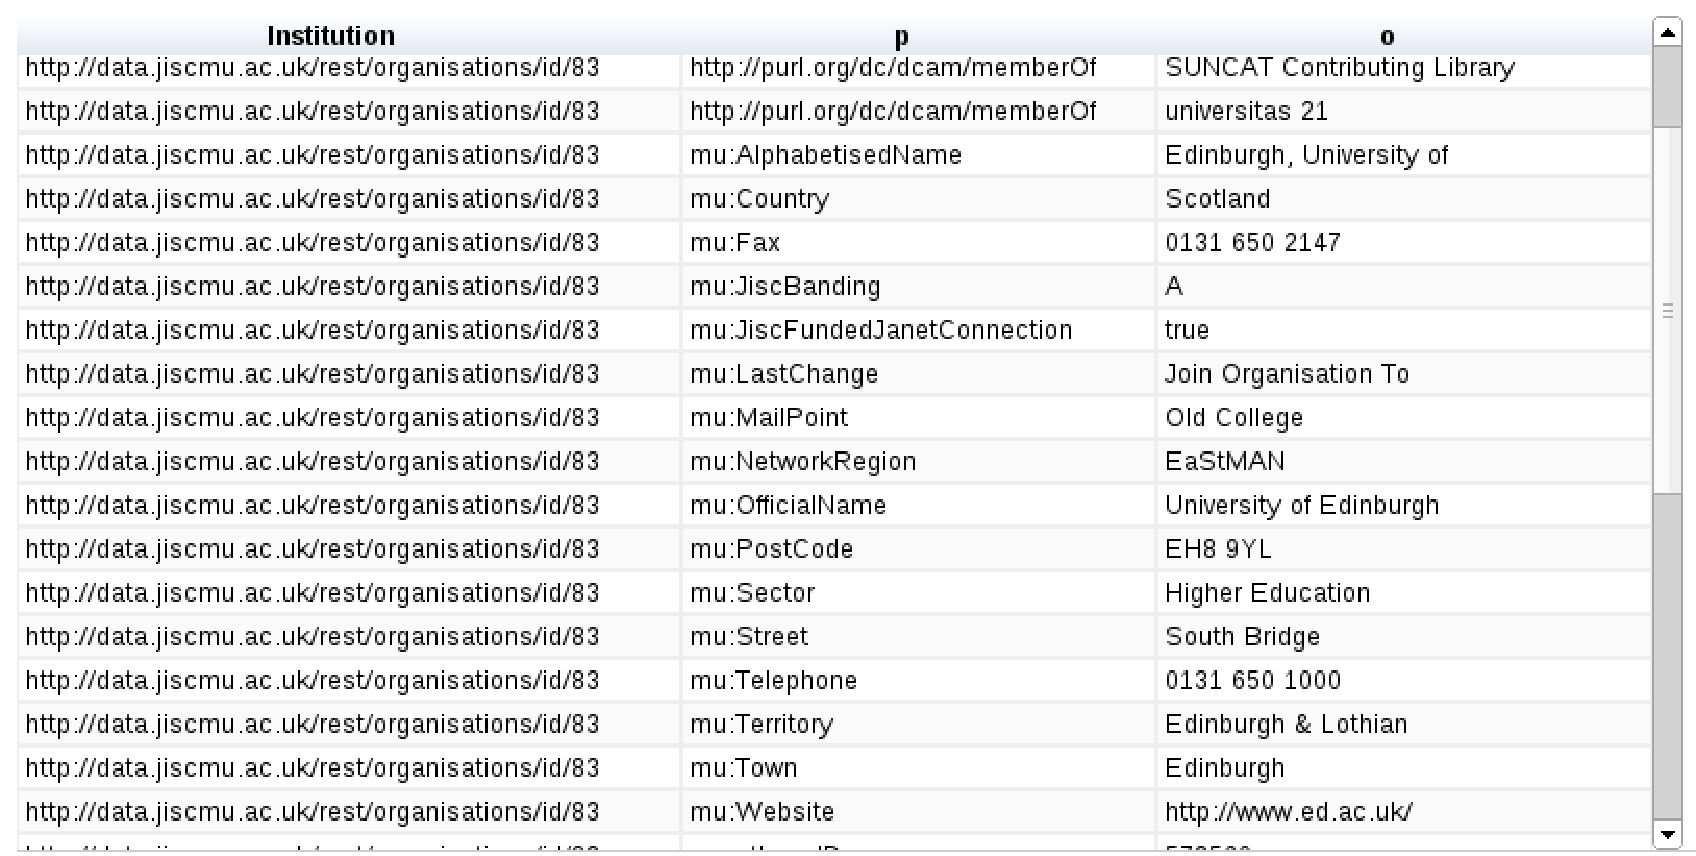
\includegraphics[width=120mm]{images/jisc-results.pdf}
\end{center}

\end{frame}


\begin{frame}

\huge
\begin{center}
Semantic Web Toolkits
\end{center}


\end{frame}


\section{Semantic Web Toolkits}

\begin{frame}
\frametitle{Semantic Web Toolkits}
\framesubtitle{Popular Toolkits}

\begin{columns}[t]
\begin{column}{0.45\textwidth}

\textbf{Functional languages}
\begin{itemize}
\item scardf (Scala)
\item Wilbur (Common Lisp)
\item Clojure-rdf (Clojure)
\item \emph{(Nothing for Erlang?)}
\end{itemize}


\end{column}

  \begin{column}{0.45\textwidth}

\textbf{(Other languages)}
\begin{itemize}
\item Jena (Java)
\item Sesame (Java)
\item Redland (C)
\item rdfquery (Javascript)
\item RAP (php)
\item SWI-Prolog (prolog)
\item Many more\ldots
\end{itemize}



 \end{column}
\end{columns}

\end{frame}

\begin{frame}
\frametitle{Jena}
\framesubtitle{A very popular semantic web framework in Java}

\begin{quotation}
`` Semantic Web applications. Jena provides a collection of tools and Java libraries to help you to develop semantic web and linked-data apps, tools and servers.''
\end{quotation}

\begin{itemize}
\item Support for serialisation of RDF in XML, N-triples and Turtle formats
\item Ontology API for handling OWL and RDFS ontologies
\item Rule-based inference engine for reasoning with RDF and OWL
\item Query engine compliant with the latest SPARQL specification
\item Lots more\ldots
\end{itemize}

\bigskip
We'll be comparing RDF4H with Jena for RDF querying and manipulation.

\end{frame}


\begin{frame}
\frametitle{Semantic Web Toolkits}
\framesubtitle{Haskell packages}

\begin{description}
\item[rdf4h] is a library for working with RDF in Haskell.
\bigskip
\item[hsparql] includes a DSL to easily create queries, as well as
  methods to submit those queries to a SPARQL server, returning the
  results as simple Haskell data structures
\bigskip
\item[swish] is another library for working with RDF in Haskell. It
  explores Haskell as "a scripting language for the Semantic
  Web".
\end{description}

\end{frame}



\begin{frame}[fragile]

\huge
\begin{center}
Haskell libraries
\end{center}

\large
\begin{center}
Looking at rdf4h
\end{center}

\begin{itemize}
\item \textbf{Author} Calvin Smith
\item \textbf{Maintainer} Rob Stewart
\item \textbf{Source code}
  
  \begin{itemize}
  \item Rob (upstream)
    
    \begin{itemize}
    \item \texttt{git clone git://github.com/robstewart57/rdf4h.git}
    \end{itemize}
    
  \end{itemize}

\end{itemize}

\end{frame}


\begin{frame}
\frametitle{Semantic Web Toolkits}
\framesubtitle{RDF4H}

\textbf{rdf4h} is a library for working with RDF in Haskell.

\begin{itemize}
\item Supports parsing and serialisation of file formats:

\begin{itemize}
\item N-Triples
\item Turtle
\item XML
\end{itemize}

\item Provides type representation of:

\begin{itemize}
\item RDF triples
\item Prefix mappings; namespaces \ldots
\end{itemize}

\item Querying over data:

\begin{itemize}
\item Sorting triples
\item Finding resources
\item Isomorphic graph equality
\item And other stuff\ldots

\end{itemize}

\end{itemize}

\end{frame}


\begin{frame}[fragile]
\frametitle{RDF4H}
\framesubtitle{Types}

\begin{haskellcode}
data Triple =
      Triple !Node !Node !Node

type Triples = [Triple]
type Subject = Node
type Predicate = Node
type Object = Node

data Node =

  -- |An RDF URI reference. See
  -- <http://www.w3.org/TR/rdf-concepts/#section-Graph-URIref> for more
  -- information.
  UNode !T.Text

  -- |An RDF blank node. See
  -- <http://www.w3.org/TR/rdf-concepts/#section-blank-nodes> for more
  -- information.
  | BNode !T.Text

  -- |An RDF blank node with an auto-generated identifier, as used in
  -- Turtle.
  | BNodeGen !Int

  -- |An RDF literal. See
  -- <http://www.w3.org/TR/rdf-concepts/#section-Graph-Literal> for more
  -- information.
  | LNode !LValue
\end{haskellcode}

\end{frame}

\begin{frame}[fragile]
\frametitle{RDF4H}
\framesubtitle{RDF type class}

\begin{haskellcode}
class RDF rdf where
  -- |Return the base URL of this graph, if any.
  baseUrl :: rdf -> Maybe BaseUrl

  -- |Return the prefix mappings defined for this graph, if any.
  prefixMappings :: rdf -> PrefixMappings

  -- |Merges specified prefix mappings with the existing mappings
  addPrefixMappings :: rdf -> PrefixMappings -> Bool -> rdf

  -- |Return an empty RDF graph.
  empty :: rdf

  -- |Return a graph containing all the given triples.
  mkRdf :: Triples -> Maybe BaseUrl -> PrefixMappings -> rdf

  -- |Return all triples in the graph, as a list.
  triplesOf :: rdf -> Triples

  -- |Return the triples in the graph that match the given pattern.
  query :: rdf -> Maybe Subject -> Maybe Predicate -> Maybe Object -> Triples
\end{haskellcode}

\end{frame}

\begin{frame}
\frametitle{RDF4H}
\framesubtitle{RDF instances}

\begin{description}
\item[TriplesGraph] contains a list-backed graph implementation
  suitable for smallish graphs or for temporary graphs that will not
  be queried. If you might have duplicate triples, use \texttt{MGraph}
  instead, which is also more efficient. 

\bigskip

\item[MGraph] A simple graph implementation backed by \texttt{Data.Map}.
\end{description}

\end{frame}

\begin{frame}[fragile]
\frametitle{RDF4H}
\framesubtitle{Useful functions}

\begin{haskellcode}
-- |Return a URIRef node for the given bytestring URI.
unode :: T.Text -> Node

-- |Return a blank node using the given string identifier.
bnode :: T.Text ->  Node

-- |Return a literal node using the given LValue.
lnode :: LValue ->  Node

-- |Constructor functions for LValue
plainL :: T.Text -> LValue
plainLL :: T.Text -> T.Text -> LValue
typedL :: T.Text -> T.Text-> LValue

-- |A constructor function for 'Triple'
triple :: Subject -> Predicate -> Object -> Triple

subjectOf :: Triple -> Node
predicateOf :: Triple -> Node
objectOf :: Triple -> Node

isIsomorphic :: forall rdf1 rdf2. (RDF rdf1, RDF rdf2) => rdf1 -> rdf2 -> Bool

\end{haskellcode}

\end{frame}


\begin{frame}[fragile]
\frametitle{Comparing RDF4H and Jena}
\framesubtitle{Reading an RDF file}


\textbf{Java}

\begin{lstlisting}[style=MyJavaStyle]
final public Model readFile(String filename) throws FileNotFoundException {
 return ModelFactory.createDefaultModel().read(new FileReader("file.nt"),null);
}
\end{lstlisting}

\bigskip
\textbf{Haskell}

\begin{haskellcode}
readRDFFile :: IO TriplesGraph
readRDFFile = fmap fromEither (parseFile NTriplesParser "file.nt")
\end{haskellcode}

\end{frame}


\begin{frame}[fragile]
\frametitle{Comparing RDF4H and Jena}
\framesubtitle{Extracting Triples from Graphs}

\textbf{Java}

\begin{lstlisting}[style=MyJavaStyle]
final public Collection<Triple> getTriples(Model model){
        Collection<Triple> triples = new LinkedList<Triple>();
        StmtIterator stmts = model.listStatements();
        Statement s;
        while (stmts.hasNext()){
            s = stmts.nextStatement();
            triples.add(s.asTriple());
        }
        return triples;
}
\end{lstlisting}

\bigskip
\textbf{Haskell}

\begin{haskellcode}
getTriples :: TriplesGraph -> Triples
getTriples graph = triplesOf graph
\end{haskellcode}


\end{frame}



\begin{frame}[fragile]
\frametitle{Comparing RDF4H and Jena}
\framesubtitle{Checking node type}

\textbf{Java}

\begin{lstlisting}[style=MyJavaStyle]
final public String checkNodeType(Node node){
        String str = null;
        if (node.isURI())         str = node + " is URI";
        else if(node.isBlank())   str = node + " is blank";
        else if(node.isLiteral()) str = node + " is literal";
        return str;
    }
\end{lstlisting}

\bigskip
\textbf{Haskell}


\begin{haskellcode}
checkNodeType :: Node -> String
checkNodeType node
  | isUNode node = (show node) ++ " is URI"
  | isBNode node = (show node) ++ " is blank"
  | isLNode node = (show node) ++ " is literal"
\end{haskellcode}

\end{frame}



\begin{frame}[fragile]
\frametitle{Comparing RDF4H and Jena}
\framesubtitle{Constructing triples with language literal}

\textbf{Java}

\begin{lstlisting}[style=MyJavaStyle]
final public Triple makeTriple(String s, String p, String oLangLiteral){
        Model model = ModelFactory.createDefaultModel();
        Node subj = model.createResource(s).asNode();
        Node pred = model.createResource(p).asNode();
        Node obj = model.createLiteral(oLangLiteral,"en").asNode();
        return new Triple(subj,pred,obj);
    }
\end{lstlisting}

\bigskip
\textbf{Haskell}

\begin{haskellcode}
mkTriple :: String -> String -> String -> Triple
mkTriple s p o = 
  let subj = unode (s2b s)
      pred = unode (s2b p)
      obj =  lnode (plainLL (s2b o) (s2b "en"))
  in triple subj pred obj
\end{haskellcode}

\end{frame}

\begin{frame}[fragile]
\frametitle{Comparing RDF4H and Jena}
\framesubtitle{Constructing RDF graphs in Java}


\begin{lstlisting}[style=MyJavaStyle,basicstyle=\scriptsize]
final public Model mkModel(){
 Model model = ModelFactory.createDefaultModel();
 String foafNS = "http://xmlns.com/foaf/0.1/";
 model.setNsPrefix("foaf", foafNS);
 Property topic_interest = model.createProperty(foafNS, "topic_interest");
 Property account = model.createProperty(foafNS, "account");

 Resource me = model.createResource("http://example.org/users/robstewart");
 Resource twitter = model.createResource("https://twitter.com/#!/robstewartUK");
 Resource haskell = model.createResource(
    "http://dbpedia.org/resource/Haskell_(programming_language)");

 Statement stmt;
 stmt = model.createStatement(me, account, twitter);
 model.add(stmt);
 stmt = model.createStatement(me, topic_interest, haskell);
 model.add(stmt);
 return model;
    }
\end{lstlisting}

\end{frame}

\begin{frame}[fragile]
\frametitle{Comparing RDF4H and Jena}
\framesubtitle{Constructing RDF graphs in Haskell}


\begin{haskellcode}
mkGraph :: TriplesGraph
mkGraph = mkRdf 
  [Triple
    ((unode . s2b) "http://example.org/users/robstewart")
    ((unode . s2b) "foaf:topic_interest")
    ((unode . s2b) "http://dbpedia.org/resource/Haskell_(programming_language)")
  ,Triple
    ((unode . s2b) "http://example.org/users/robstewart")
    ((unode . s2b) "foaf:account")
    ((unode . s2b) "https://twitter.com/#!/robstewartUK")
  ]
  Nothing
  (PrefixMappings
    (Map.fromList [ (s2b "foaf", s2b "http://xmlns.com/foaf/0.1/") ]))
\end{haskellcode}

\end{frame}


\begin{frame}

\huge
\begin{center}
Haskell libraries
\end{center}

\large
\begin{center}
Looking at swish
\end{center}

\begin{itemize}
\item \textbf{Author} Graham Klyne
\item \textbf{Maintainers} Doug Burke
\item \textbf{Source code}
  
  \begin{itemize}
  \item Doug
    
    \begin{itemize}
    \item \texttt{hg clone https://bitbucket.org/doug\_burke/swish}
    \end{itemize}
    
  \end{itemize}
  
\end{itemize}

\end{frame}

\begin{frame}[fragile]
\frametitle{Semantic Web Toolkits}
\framesubtitle{A quick look at Swish}

Homepage: \texttt{http://www.ninebynine.org/RDFNotes/Swish/Intro.html}


\begin{itemize}

\item Haskell framework for performing deductions on RDF data
\item Graph isomorphism equality and differences
\item Inference engine
  
  \begin{itemize}
  \item Forward chain reasoning
  \item Backward chain reasoning
  \item Proof checking module
  \end{itemize}
  
\item Horn-style rule implementations
\item RDF formal semantics entailment rule implementation
\item Ready-to-run command line and script-driven programs
  
\end{itemize}


\end{frame}


\begin{frame}

\huge
\begin{center}
Haskell libraries
\end{center}

\large
\begin{center}
Looking at hsparql
\end{center}

\begin{itemize}
\item \textbf{Author} Jeff Wheeler
\item \textbf{Maintainer} Rob Stewart
\item \textbf{Source code}

\begin{itemize}
\item \texttt{git clone git://github.com/robstewart57/hsparql.git}
\end{itemize}

\end{itemize}

\end{frame}


\begin{frame}[fragile]
\frametitle{Hsparql}
\framesubtitle{hsparql}

\textbf{hsparql} includes a SPARQL domain specific language\ldots

\begin{itemize}
\item Programmatically create SPARQL queries
  
\item Includes functions for submitting SPARQL queries
  
  \begin{itemize}
  \item For \texttt{CONSTRUCT, SELECT, DESCRIBE} and \texttt{ASK} queries
  \end{itemize}
  
\item Includes SPARQL response data structures
  
  \begin{itemize}
  \item SPARQL Query Solutions (for \texttt{select} and \texttt{ask} queries)
  \item RDF graphs (for \texttt{describe} and \texttt{construct}
    queries)

    \begin{itemize}
    \item Adopting the types from the `rdf4h' package
    \end{itemize}

  \end{itemize}

\end{itemize}

\end{frame}

\begin{frame}
\frametitle{Hsparql}
\framesubtitle{Flow}

\begin{center}
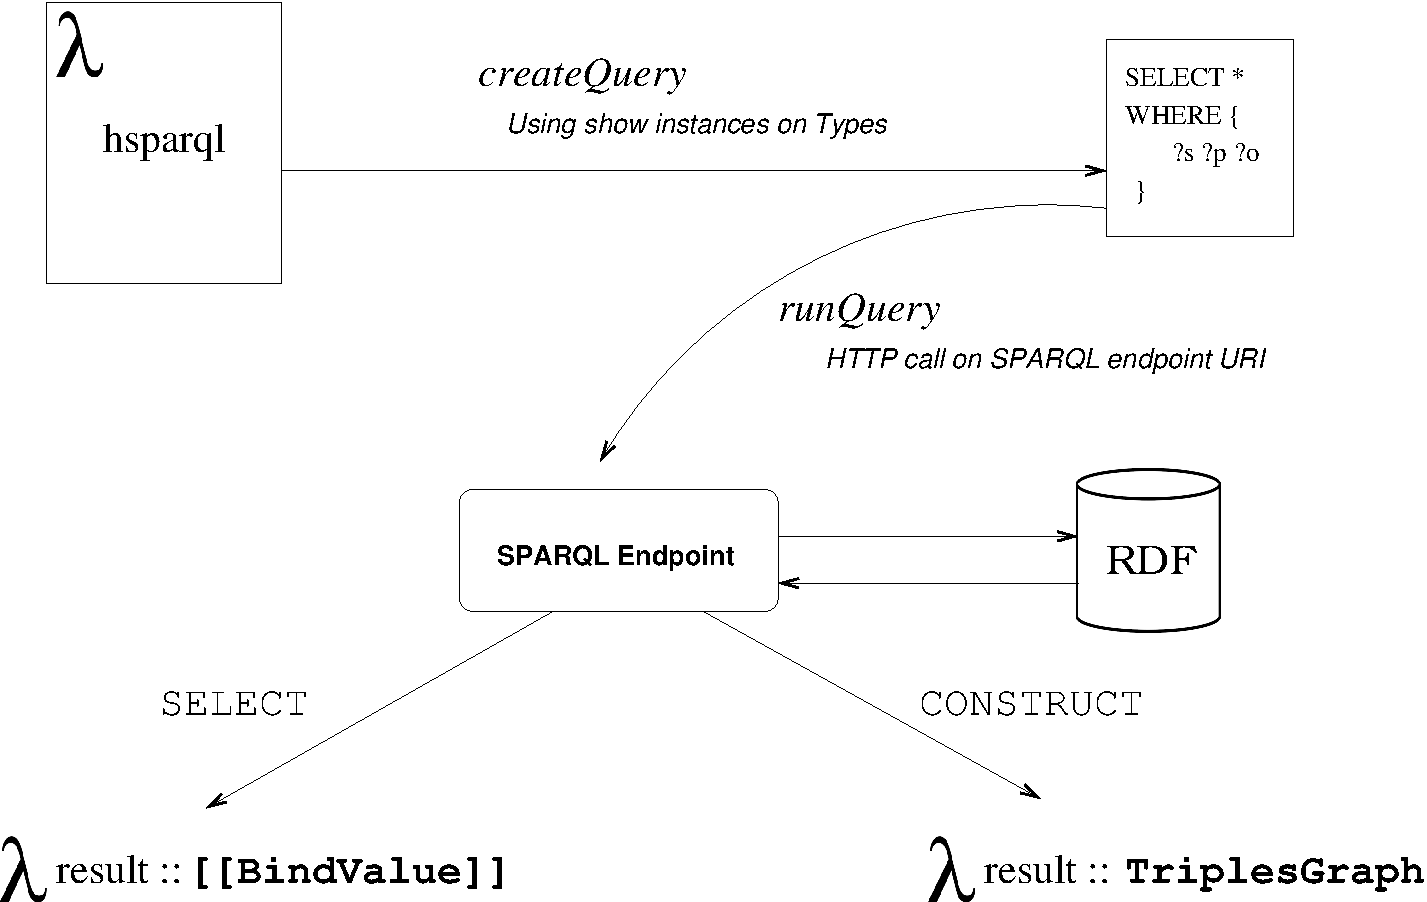
\includegraphics[width=110mm]{images/hsparql-flow.pdf}
\end{center}


\end{frame}

\begin{frame}[fragile]
\frametitle{Hsparql}
\framesubtitle{Generating SPARQL Queries - Types}

\begin{haskellcode}
data Duplicates = NoLimits | Distinct | Reduced

data Prefix = Prefix String IRIRef

data IRIRef = IRIRef String
            | PrefixedName Prefix String 

data RDFLiteral = RDFLiteral String
                | RDFLiteralLang String String
                | RDFLiteralIRIRef String IRIRef

data Relation = Equal | NotEqual | LessThan | GreaterThan
       | LessThanOrEqual | GreaterThanOrEqual

data Operation = Add | Subtract | Multiply | Divide

data OrderBy = Asc Expr
             | Desc Expr
\end{haskellcode}

\end{frame}

\begin{frame}[fragile]
\frametitle{Hsparql}
\framesubtitle{Generating SPARQL Queries - Types}

\begin{haskellcode}
-- |Permit variables and values to seamlessly be put into 'triple'
-- class TermLike a where

data QueryType = SelectType | ConstructType | TypeNotSet

data QueryForm = SelectForm QueryData | ConstructForm QueryData

-- |Local representations of incoming XML results.
data BindingValue = Bound Data.RDF.Node    -- ^RDF Node (UNode, BNode, LNode)
                  | Unbound       -- ^Unbound result value
  deriving (Show, Eq)


data ConstructQuery = ConstructQuery
    { queryConstructs :: [Pattern] }

data SelectQuery = SelectQuery
    { queryVars :: [Variable] }
\end{haskellcode}

\end{frame}


\begin{frame}[fragile]
\frametitle{Hsparql}
\framesubtitle{Examples of show instances}

\begin{haskellcode}
instance QueryShow Relation where
  qshow Equal              = "="
  qshow NotEqual           = "!="
  qshow LessThan           = "<"
  qshow GreaterThan        = ">"
  qshow LessThanOrEqual    = "<="
  qshow GreaterThanOrEqual = ">="

instance QueryShow OrderBy where
  qshow (Asc e)  = "ASC(" ++ qshow e ++ ")"
  qshow (Desc e) = "DESC(" ++ qshow e ++ ")"

instance QueryShow QueryForm where
  qshow (SelectForm qd) =  unwords 
                        [ "SELECT"
                         , qshow (duplicates qd)
                         , qshow (vars qd)
                        ]

  qshow (ConstructForm qd) = "CONSTRUCT { " ++ qshow (constructTriples qd) ++ " }"
\end{haskellcode}
\end{frame}

\begin{frame}[fragile]
\frametitle{Hsparql}
\framesubtitle{Generating a simple \texttt{SELECT} query}

\scriptsize
\begin{verbatim}
PREFIX resource: <http://dbpedia.org/resource/>
PREFIX dbprop: <http://dbpedia.org/property/>
PREFIX foaf: <http://xmlns.com/foaf/0.1/>
SELECT ?name ?page
WHERE {
  ?x dbprop:genre resource:Web_browser .
  ?x foaf:name ?name .
  ?x foaf:page ?page .
}
\end{verbatim}
\end{frame}

\begin{frame}[fragile]
\frametitle{Hsparql}
\framesubtitle{Generating a simple \texttt{SELECT} query}

\scriptsize
\begin{verbatim}
simpleSelect :: Query SelectQuery
simpleSelect = do
    resource <- prefix "dbprop" (iriRef "http://dbpedia.org/resource/")
    dbpprop  <- prefix "dbpedia" (iriRef "http://dbpedia.org/property/")
    foaf     <- prefix "foaf" (iriRef "http://xmlns.com/foaf/0.1/")

    x    <- var
    name <- var
    page <- var

    triple x (dbpprop .:. "genre") (resource .:. "Web_browser")

    triple x (foaf .:. "name") name
    triple x (foaf .:. "page") page

    return SelectQuery { queryVars = [name, page] }
\end{verbatim}
\end{frame}

\begin{frame}[fragile]
\frametitle{Hsparql}
\framesubtitle{Generating a simple \texttt{CONSTRUCT} query}

\scriptsize
\begin{verbatim}
simpleConstruct :: Query ConstructQuery
simpleConstruct = do
    resource <- prefix "dbpedia" (iriRef "http://dbpedia.org/resource/")
    dbpprop  <- prefix "dbprop" (iriRef "http://dbpedia.org/property/")
    foaf     <- prefix "foaf" (iriRef "http://xmlns.com/foaf/0.1/")
    example  <- prefix "example" (iriRef "http://www.example.com/")

    x    <- var
    name <- var
    page <- var

    construct <- constructTriple x (example .:. "hasName") name
    
    triple x (dbpprop .:. "genre") (resource .:. "Web_browser")
    triple x (foaf .:. "name") name
    triple x (foaf .:. "page") page

    return ConstructQuery { queryConstructs = [construct] }
\end{verbatim}
\end{frame}


\begin{frame}[fragile]
\frametitle{Hsparql Under The Hood}
\framesubtitle{Submitting SPARQL SELECT query}

\scriptsize
\begin{alltt}
-- |Transform the 'String' result from the HTTP request into a two-dimensional
--  table storing the bindings for each variable in each row.
\hilightyellow{structureContent :: String -> Maybe [[BindingValue]]}

-- |Connect to remote 'EndPoint' and find all possible bindings for the
--  'Variable's in the 'SelectQuery' action.
selectQuery :: EndPoint -> Query SelectQuery -> IO (Maybe [[BindingValue]])
selectQuery ep q = do
    let uri      = ep ++ "?" ++ urlEncodeVars [("query", \hilightyellow{createSelectQuery q})]
        request  = replaceHeader HdrUserAgent "hsparql-client" (getRequest uri)
    \hilightyellow{response <- simpleHTTP request >>= getResponseBody}
    return (\hilightyellow{structureContent response})
\end{alltt}

\end{frame}

\begin{frame}[fragile]
\frametitle{Hsparql Under The Hood}
\framesubtitle{Submitting SPARQL CONSTRUCT query}

\scriptsize
\begin{alltt}
-- |Connect to remote 'EndPoint' and construct 'TriplesGraph' from given
--  'ConstructQuery' action. /Provisional implementation/.
constructQuery :: forall rdf. (RDF rdf) =>
   Database.HSparql.Connection.EndPoint -> Query ConstructQuery -> IO rdf
constructQuery ep q = do
    let uri      = ep ++ "?" ++ urlEncodeVars [("query", createConstructQuery q)]
    rdfGraph <- httpCallForRdf uri
    case rdfGraph of
      Left e -> error $ show e
      Right graph -> return graph

httpCallForRdf :: RDF rdf => String -> IO (Either ParseFailure rdf)
httpCallForRdf uri = do
  let h1 = mkHeader HdrUserAgent "hsparql-client"
      h2 = mkHeader HdrAccept "text/turtle"
      request = Request { rqURI = fromJust $ parseURI uri
                          , rqHeaders = [h1,h2]
                          , rqMethod = GET
                          , rqBody = ""
                          }
  response <- simpleHTTP request >>= getResponseBody
  let content = E.decodeUtf8 (B.pack response)
  return \$ parseString (TurtleParser Nothing Nothing) content
\end{alltt}

\end{frame}


\begin{frame}[fragile]
\frametitle{Hsparql}
\framesubtitle{Hsparql in use}

\scriptsize
\begin{verbatim}
selectExample :: IO ()
selectExample = do
  (Just s) <- selectQuery "http://dbpedia.org/sparql" simpleSelect
  putStrLn . take 500 . show $ s

askExample :: IO ()
askExample = do
  res <- askQuery "http://dbpedia.org/sparql" simpleAsk
  putStrLn $ "result: " ++ show (res::Bool)

describeExample :: IO ()
describeExample = do
  rdfGraph <- describeQuery "http://dbpedia.org/sparql" simpleDescribe
  mapM_ print (triplesOf rdfGraph)

constructExample :: IO ()
constructExample = do
  rdfGraph <- constructQuery "http://dbpedia.org/sparql" simpleConstruct
  mapM_ print (triplesOf rdfGraph)
\end{verbatim}

\end{frame}


\begin{frame}[fragile]
\frametitle{Hsparql}
\framesubtitle{A more interesting \texttt{SELECT} example\ldots}

\tiny
\begin{verbatim}
berliners :: Query SelectQuery
berliners = do
    xsd  <- prefix "xsd" (iriRef "http://www.w3.org/2001/XMLSchema#")
    prop <- prefix "prop" (iriRef "http://dbpedia.org/property/")
    dbo  <- prefix "dbo" (iriRef "http://dbpedia.org/ontology/")
    foaf <- prefix "foaf" (iriRef "http://xmlns.com/foaf/0.1/")
    resc <- prefix "resc" (iriRef "http://dbpedia.org/resource/")

    name     <- var
    birth    <- var
    death    <- var
    person   <- var
    knownfor <- var

    triple person (prop .:. "birthPlace") (resc .:. "Berlin")
    triple person (dbo  .:. "birthdate")  birth
    triple person (foaf .:. "name")       name
    triple person (dbo  .:. "deathdate")  death

    filterExpr $ birth .<. ("1900-01-01", xsd .:. "date")

    optional $ triple person (prop .:. "KnownFor") knownfor

    return SelectQuery { queryVars = [name, birth, death, person, knownfor] }
\end{verbatim}

\end{frame}


\begin{frame}[fragile]
\frametitle{Hsparql}
\framesubtitle{A more interesting \texttt{SELECT} example \emph{result}}

\scriptsize
\begin{verbatim}
[
 [LangLiteral "Wilhelm II" "en",
  TypedLiteral "1859-01-27" "http://www.w3.org/2001/XMLSchema#date",
  TypedLiteral "1941-06-04" "http://www.w3.org/2001/XMLSchema#date",
  URI "http://dbpedia.org/resource/Wilhelm_II,_German_Emperor",
  Unbound]
,[LangLiteral "German Emperor Wilhelm II" "en",
  TypedLiteral "1859-01-27" "http://www.w3.org/2001/XMLSchema#date",
  TypedLiteral "1941-06-04" "http://www.w3.org/2001/XMLSchema#date",
  URI "http://dbpedia.org/resource/Wilhelm_II,_German_Emperor",
  Unbound]
,[LangLiteral "Edmund Landau" "en",
  TypedLiteral "1877-02-14" "http://www.w3.org/2001/XMLSchema#date",
  TypedLiteral "1938-02-19" "http://www.w3.org/2001/XMLSchema#date",
  URI "http://dbpedia.org/resource/Edmund_Landau",
  Unbound]
]
\end{verbatim}

\end{frame}


\begin{frame}[fragile]
\frametitle{Hsparql}
\framesubtitle{Another interesting \texttt{SELECT} example\ldots}

\tiny
\begin{verbatim}
selectExample :: IO ()
selectExample = do
  (Just s) <- selectQuery "http://api.talis.com/stores/bbc-backstage/services/sparql" drWhoQuery
  putStrLn . show $ s

drWhoQuery :: Query SelectQuery
drWhoQuery = do
  rdfs <- prefix "rdfs" (iriRef "http://www.w3.org/2000/01/rdf-schema#")
  po  <- prefix "po" (iriRef "http://purl.org/ontology/po/")
  dc    <- prefix "dc" (iriRef "http://purl.org/dc/elements/1.1/")

  position <- var
  title    <- var
  syn      <- var
  series   <- var
  episode  <- var

  triple (iriRef "http://www.bbc.co.uk/programmes/b006q2x0#programme") (po .:. "series") series
  triple series (dc .:. "title") "Series 3"
  triple series (po .:. "episode") episode

  triple episode (dc .:. "title") title
  triple episode (po .:. "position") position
  triple episode (po .:. "short_synopsis") syn

  return SelectQuery { queryVars = [position, title, syn] }
\end{verbatim}

\end{frame}


\begin{frame}
\frametitle{Hsparql}
\framesubtitle{Dr Who results}

\begin{center}

\scriptsize
\begin{tabular}{| c | c | >{\tiny}p{5.5cm} |}
\hline
\textbf{Position} & \textbf{Title} & \textbf{Syn} \\
\hline
6 & The Lazarus Experiment & Martha has to save her family from the
schemes of the monstrous Professor Lazarus. \\
13 & Last of the Time Lords & Earth has been conquered and the Master
rules supreme. Can Martha Jones save the world? \\
2 & The Shakespeare Code & In Elizabethan England, William Shakespeare
is under the control of witch-like creatures. \\
10 & Blink & Only the Doctor can stop the Weeping Angels, but he's
lost in time. \\
5 & Evolution of the Daleks & As a new Dalek Empire rises in 1930s New
York, the Doctor must enter an unholy alliance. \\
4 & Daleks in Manhattan & The Doctor finds his oldest enemies at work
on top of the Empire State Building. \\
7 & 42 & The Doctor and Martha have to stop a spaceship from hurtling
into the sun. \\
8 & Human Nature & A schoolteacher called John Smith dreams of
adventures in time and space. \\
11 & Utopia & Captain Jack Harkness storms back into the Doctor's
life. \\
12 & The Sound of Drums & Harry Saxon becomes Prime Minister, but his
dark ambitions reach beyond the stars. \\
1 & Smith and Jones & When Martha Jones finds herself on the moon, she
meets a stranger called the Doctor. \\
3 & Gridlock & The Doctor takes Martha to New Earth, only to find that
the city has become a deadly trap. \\
9 & The Family of Blood & It's 1913 and war comes to England early, as
the terrifying Family hunt for the Doctor. \\
\hline
\end{tabular}
\end{center}

\end{frame}

\section{Conclusion}

\begin{frame}

\huge
\begin{center}
A Plan?
\end{center}

\end{frame}

\begin{frame}[fragile]
\frametitle{Towards a Semantic Web Toolkit for Haskell}
\framesubtitle{Future Work}

\begin{itemize}
\item rdf4h
  
  \begin{itemize}
  \item Move towards feature parity with Jena Models
  \end{itemize}
  
\item swish
  
  \begin{itemize}
  \item Complete UTF-8 handling
  \item Internals: move to \emph{polyparse, LookupMap}\ldots
  \end{itemize}
  
\item hsparql
\scriptsize
\begin{verbatim}
askQuery      :: EndPoint -> Query AskQuery -> IO Bool
describeQuery :: EndPoint -> Query DescribeQuery -> IO TriplesGraph
\end{verbatim}
\normalsize

  \bigskip
\item A unified semantic web Type representation!
  
  \begin{itemize}
  \item Have all 3 packages use the same representations
\begin{itemize}
\item \emph{prefix mappings, URIs, typed literals\ldots}
\end{itemize}
  
\item Unified serialisation of XML, N3, Turtle

    
  \end{itemize}
  
\end{itemize}

\end{frame}

\begin{frame}
\frametitle{Towards a Semantic Web Toolkit}
\framesubtitle{A place for Haskell in the Semantic Web}

\begin{itemize}
\item A feature rich RDF library
  
  \begin{itemize}
  \item Providing an array of high level APIs working with RDF
  \end{itemize}
  
  \begin{center}\textbf{and}\end{center}
  
\item SPARQL construction \& execution
  
  \begin{itemize}
  \item \emph{Programmatically} generate and execute SPARQL
    queries\ldots
  \item Living within the Haskell type system along the way
  \end{itemize}
  
  \begin{center}\textbf{and}\end{center}
  
\item A scripting interface to IO with RDF
  
  \begin{itemize}
  \item To read, write \& merge RDF graphs
  \item Apply forward and backward chain reasoning rule inference
  \item Compare graphs for equality
    
  \end{itemize}
  
\end{itemize}

\end{frame}

\begin{frame}

\huge
\begin{center}
The end.
\end{center}

\end{frame}


\end{document}
